
\documentclass[12pt]{iopart}
\pdfoutput=1
\usepackage{iopams}
\usepackage{amssymb, epsfig}
%\usepackage{amsmath, amssymb,epsfig}
\usepackage{latexsym}

%\usepackage[hypertex,hyperindex]{hyperref}
%\usepackage{showkeys}
\usepackage{graphicx}
\usepackage{color}

\newcommand{\pf}{\mbox{pf}}

\begin{document}
	
	\bibliographystyle{plain}
	\def\debproof{\noindent {\bf Proof.} }
	\def\finproof{\hfill {\small $\Box$} \\}
	%\renewcommand{\theequation}{\arabic{section}.\arabic{equation}}
	
	\makeatletter % `@' now normal "letter"
	\@addtoreset{equation}{section}
	\makeatother  % `@' is restored as "non-letter"
	\renewcommand\theequation{{\thesection}.{\arabic{equation}}}
	\title[]{}
	
	
	
	\maketitle
	\newcommand{\eps}{\varepsilon}
	\newcommand{\RR}{\mathcal{R}}
	\newtheorem{lem}{Lemma}[section]
	\newtheorem{prop}{Proposition}[section]
	\newtheorem{cor}{Corollary}[section]
	\newtheorem{thm}{Theorem}[section]
	\newtheorem{rem}{Remark}[section]
	\newtheorem{alg}{Algorithm}[section]
	\newtheorem{assum}{Assumption}[section]
	\newtheorem{definition}{Definition}[section]
	
	
	\newcounter{RomanNumber}
	\newcommand{\MyRoman}[1]{\rm\setcounter{RomanNumber}{#1}\Roman{RomanNumber}}
	
	\newcommand{\bL}{\mathbf{L}}
	\newcommand{\bH}{\mathbf{H}}
	\newcommand{\bW}{\mathbf{W}}
	\newcommand{\bP}{\mathbf{P}}
	\newcommand{\bQ}{\mathbf{Q}}
	\newcommand{\bp}{\mathbf{p}}
	\newcommand{\bq}{\mathbf{q}}
	\newcommand{\uL}{u_{_{\rm L}}}
	\newcommand{\vL}{v_{_{\rm L}}}
	\newcommand{\tuL}{\tilde u_{_{\rm L}}}
	\newcommand{\tvL}{\tilde v_{_{\rm L}}}
	\newcommand{\fL}{f_{_{\rm L}}}
	\newcommand{\gL}{g_{_{\rm L}}}
	\newcommand{\bpL}{\bp_{_{\rm L}}}
	\newcommand{\bqL}{\bq_{_{\rm L}}}
	\newcommand{\tbpL}{\tilde{\bp}_{_{\rm L}}}
	\newcommand{\tbqL}{\tilde{\bq}_{_{\rm L}}}
	\newcommand{\tbpLf}{\tilde{\bp}_{_{\rm L,1}}}
	\newcommand{\tbpLs}{\tilde{\bp}_{_{\rm L,2}}}
	\newcommand{\tbqLf}{\tilde{\bq}_{_{\rm L,1}}}
	\newcommand{\tbqLs}{\tilde{\bq}_{_{\rm L,2}}}
	\newcommand{\bn}{\nu}
	\newcommand{\bv}{\mathbf{v}}
	\newcommand{\om}{\omega}
	\newcommand{\pa}{\partial}
	\newcommand{\la}{\langle}
	\newcommand{\ra}{\rangle}
	\newcommand{\lla}{\la{\hskip -2pt}\la}
	\newcommand{\rra}{\ra{\hskip -2pt}\ra}
	\newcommand{\jj}{\|{\hskip -0.8pt} |}
	\newcommand{\al}{\alpha}
	\newcommand{\ze}{\zeta}
	\newcommand{\si}{\sigma}
	\newcommand{\ep}{\varepsilon}
	\newcommand{\na}{\nabla}
	\newcommand{\vp}{\varphi}
	\newcommand{\ga}{\gamma}
	\newcommand{\Ga}{\Gamma}
	\newcommand{\Om}{\Omega}
	\newcommand{\de}{\delta}
	\newcommand{\Th}{\Theta}
	\newcommand{\De}{\Delta}
	\newcommand{\Lam}{\Lambda}
	\newcommand{\lam}{\lambda}
	\newcommand{\tri}{\triangle}
	\newcommand{\lj}{[{\hskip -2pt} [}
	\newcommand{\rj}{]{\hskip -2pt} ]}
	\newcommand{\bks}{\backslash}
	%\newcommand{\diag}{\mathrm{diag}}
	\newcommand{\diam}{\mathrm{diam}}
	\newcommand{\osc}{\mathrm{osc}}
	\newcommand{\meas}{\mathrm{meas}}
	\newcommand{\dist}{\mathrm{dist}}
	
	\newcommand{\mL}{\mathscr{L}}
	\newcommand{\cT}{{\cal T}}
	\newcommand{\cM}{{\cal M}}
	\newcommand{\cE}{{\cal E}}
	\newcommand{\cL}{{\cal L}}
	\newcommand{\cF}{{\cal F}}
	\newcommand{\cB}{{\cal B}}
	\newcommand{\PML}{{\rm PML}}
	\newcommand{\FEM}{{\rm FEM}}
	\newcommand{\rd}{\,\mathrm{d}}
	
	\renewcommand{\i}{\mathbf{i}}
	\renewcommand{\v}{\mathbf{v}}
	\renewcommand{\u}{\mathbf{u}}
	\renewcommand{\r}{\mathbf{r}}
	\newcommand{\R}{{\mathbb{R}}}
	\newcommand{\Z}{{\mathbb{Z}}}
	\newcommand{\C}{{\mathbb{C}}}
	\renewcommand{\Re}{\mathrm{Re}\,}
	\renewcommand{\Im}{\mathrm{Im}\,}
	\renewcommand{\div}{\mathrm{div}}
	\newcommand{\curl}{\mathrm{curl}}
	\newcommand{\Curl}{\mathbf{curl}}
	
	
	%%%%%%%%%%%%%%%%%%%%%%%%%%%%%%%%%%%%%%%%%%%%%%%%%%%%%%%%%%%%%%%%%%%%
	\newcommand{\be}{\begin{eqnarray}}
	\newcommand{\ee}{\end{eqnarray}}
	\newcommand{\ben}{\begin{eqnarray*}}
		\newcommand{\een}{\end{eqnarray*}}
	\newcommand{\nn}{\nonumber}
	
	


\section{New proof for Stationary Phase Method}
Preminary:
\ben
\cos\theta=1-2\sin^2\frac{\theta}{2}:=1-t^2\\
t=e^{-\i\frac{\pi}{4}}s\\
\sin\theta(s):=S(s)=e^{-\i\frac{\pi}{4}}s(2+\i s^2)^{-1/2}\cos\phi+(1+\i s^2)\sin\phi \\
\cos\theta(s):=C(s)=(1+\i s^2)\cos\phi-e^{-\i\frac{\pi}{4}}s(2+\i s^2)^{-1/2}\sin\phi \\
\cos\frac{\theta(s)}{2}=(2-(t(s))^2)^{1/2}=(2+\i s^2)^{1/2}
\een

Let $f(\xi):=h(\xi,\mu(\xi),\mu_\kappa(\xi))$ be a analytic function with respect to $\xi$ in $\C\bks\{\i\R\cup(-1,1)\}$. For any $a,b>0$, we denote
\ben
I(f;a,b)=\int_{\R}f(\xi)e^{\i a\xi+\i b\mu(\xi)}d\xi
\een
where $\mu(\xi)=(1-\xi^2)^{1/2}$, $\mu_\kappa(\xi)=(\kappa-\xi^2)^{1/2}$.
\begin{lem}\label{new_station_phase}
	Let $a,b >0$, $\rho=\sqrt{a^2+b^2}$, and $f(\xi):=h(\xi,\mu(\xi),\mu_\kappa(\xi))$ be a analytic function in $\C\bks\{\i\R\cup(-1,1)\}$. Then 
	\ben\hspace{-2.5cm}
	I(f;a,b)=\sqrt{\frac{2}{\rho}}e^{\i\rho-\i\pi/4}\int_{\R}F(\frac{t}{\sqrt{\rho}})C(\frac{t}{\sqrt{\rho}})e^{-t^2}dt+
	O(\rho^{-3/2})\|F(\frac{t}{\sqrt{\rho}})C(\frac{t}{\sqrt{\rho}})t^2e^{-t^2}\|_{L^1(\R)}
	\een
	where $F(s)= h(S(s),C(s),\mu_\kappa(S(s))$ and $\sin\phi=a/\rho,\cos\phi=b/\rho$.
\end{lem}
\debproof
 To simplify the integral, the standard substitution $\xi=k_s\sin \theta$ is made, taking the $\xi$-plane to a strip $-\pi/2<\Re \theta <\pi/2$ in the $\theta$-plane, and the real axis in the $\xi$-plane onto the path L from $-\pi/2+\i\infty\rightarrow-\pi/2\rightarrow\pi/2\rightarrow\pi/2-\i\infty$ in the $\theta-plane$. The integral $I(f;a,b)$ then becomes( Let a=$\rho \sin\phi$  and b=$\rho\cos\phi$, $0<\phi<\pi/2$)
\be
 I(f;a,b)=\int_L h(\sin \theta,\cos \theta,\mu_\kappa(\sin \theta))\cos \theta \ e^{\i\rho(\cos (\theta-\phi))} d\theta
\ee
Taking the shift transformation of $\theta$ and using cauchy integral theorem, we can obtain the more useful representation of $I(f;a,b)$:
\be
I(f;a,b)=\int_L f(\sin (\theta+\phi))\cos (\theta+\phi) \ e^{\i\rho\cos \theta} d\theta
\ee
\begin{figure}
	\centering
	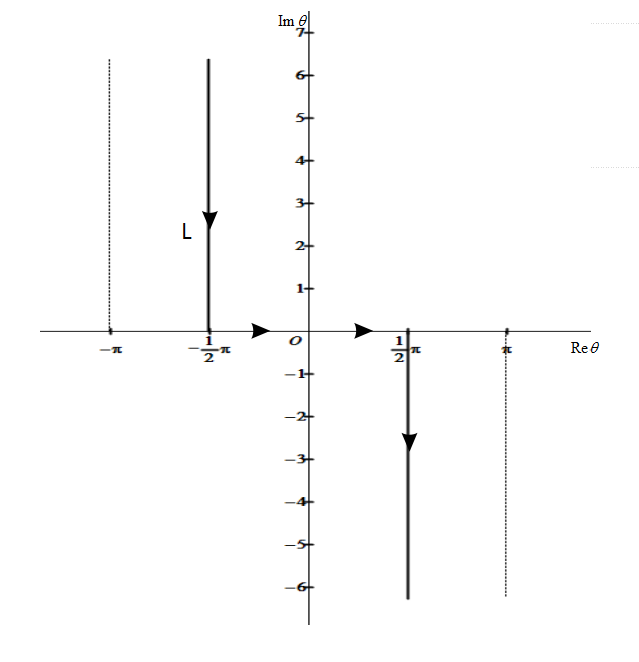
\includegraphics[width=0.4\textwidth]{./graphic/transform_th.png}
	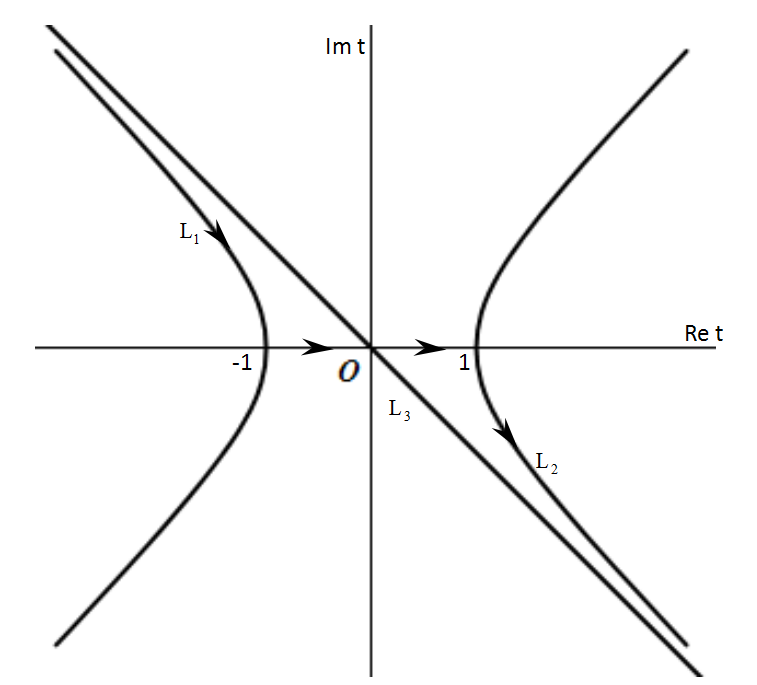
\includegraphics[width=0.4\textwidth]{./graphic/transform_t.png}

	\caption{integral path in $\theta-plane$ and t-plane  }\label{transform_t}
\end{figure}
Notice that $\cos\theta=1-2\sin^2\frac{\theta}{2}$, by substituting $\theta(t)=2\arctan\frac{\sqrt{2}t}{2}$, we get:
\ben\hspace{-1.5cm}
I(f;a,b)=e^{\i\rho}\int_{L_1\cup(-1,1)\cup L_2} f(\sin (\theta(t)+\phi))\cos (\theta(t)+\phi)\frac{2}{(2-t^2)^{1/2}} \ e^{-\i\rho t^2} dt
\een
where 
\ben
L1=\{t|(\Re t)^2-(\Im t)^2=1,\Re t <0,\Im t>0\}\\
L2=\{t|(\Re t)^2-(\Im t)^2=1,\Re t >0,\Im t<0\}
\een
and the geometry is depicted in Figure \ref{transform_t}. A simple computation show that the substitution $\theta(t)=2\arctan\frac{\sqrt{2}t}{2}$ transform the domain $\Omega_\theta=\{\theta||\Re\theta|<\pi, \Re\theta\cdot\Im\theta<0\}$ in the $\theta$-plane into $\Omega_t=\{t| \Re t\cdot\Im t<0\}$ in t-plane. Now it is easy to see that $f(\sin(\theta(t)_\phi))$ is analytic in the domain $\Omega_t$. Since $\Omega_t$ is surrounded by $L_1\cup L_2\cup(-1,1)$ and the diagonal line of the second and the fourth quadrants denote by $L3$, by using Cauchy integral theorem, we have
\ben\hspace{-1.5cm}
I(f;a,b)=e^{\i\rho}\int_{L_3} f(\sin (\theta(t)+\phi))\cos (\theta(t)+\phi)\frac{2\cos (\theta(t)+\phi)}{(2-t^2)^{1/2}} \ e^{-\i\rho t^2} dt \\ \hspace{-1.5cm}
=e^{\i\rho-\i \pi/4}\int_{\R} f(\sin (\theta(e^{-\i\pi/4 s})+\phi))\frac{2\cos (\theta(e^{-\i\pi/4 s})+\phi)}{(2+\i s^2)^{1/2}} \ e^{-\rho s^2} ds \\
 \hspace{-1.5cm}
=e^{\i\rho-\i \pi/4}\int_{\R} f(S(s))\frac{2C(s)}{(2+\i s^2)^{1/2}} \ e^{-\rho s^2} ds \\
\hspace{-1.5cm}
=\sqrt{\frac{2}{\rho}}e^{\i\rho-\i \pi/4}\int_{\R} f(S(\frac{t}{\sqrt{\rho}}))C(\frac{t}{\sqrt{\rho}}){(1+\i \frac{t^2}{2\rho})^{-1/2}} \ e^{-t^2} dt
\een
The lemma follows immediately from the fact that $(1+\i s)^{-1/2}=1+O(|s|),s\in\R$. The proof is completed.
\finproof
The following lemma is a directed consequence of lemma \ref{new_station_phase}
\begin{lem}
	Let p(x,y,z) be a homogeneous polynomial of degree 2 and $f(\xi)=p(\xi,\mu(\xi),\mu_\kappa(\xi))/(\xi^2+\mu(\xi)\mu_\kappa(\xi))$. Then for $\rho>1$, we have
	\ben
	|I(f;a,b)|\leq C(\frac{b}{\rho}\rho^{-1/2}+\frac{a}{\rho}\rho^{-5/4}+\rho^{-3/2})
	\een
	where C is a constant independant of $a,b$.
\end{lem}
\debproof
By lemme \ref{new_station_phase}, it suffice to estimate the integral $I(\rho)$ where
\ben
I(\rho)=\int_{\R}F(\frac{t}{\sqrt{\rho}})C(\frac{t}{\sqrt{\rho}})e^{-t^2}dt \\
= \cos\phi\int_{\R}F(\frac{t}{\sqrt{\rho}})(1+\i\frac{t^2}{\rho})e^{-t^2}dt-\frac{1}{\rho}\sin\phi\int_{\R}e^{-\i\pi/4} F(\frac{t}{\sqrt{\rho}})(2+\i\frac{t^2}{\rho})^{1/2}te^{-t^2}dt \\
:=\frac{b}{\rho}\phi I_1(\rho)-\frac{1}{\rho}\frac{a}{\rho} e^{-\i\pi/4} I_2(\rho)
\een
For $s\in\R$, it is easy to check that
\ben
\max\{|S(s)|,|C(s)|\}\leq |s(2+\i s^2)^{1/2}|+|1+\i s^2|\leq C(1+s+s^2)\\
|\mu_\kappa(C(s))|\leq C(1+|S(s)|)\leq C (1+s+s^2) 
\een
where C is independent of $\phi$. Consequently, for $\rho>1$, we obtain
\ben
|I_1(\rho)|\leq\int_\R |p(S(\frac{t}{\sqrt{\rho}}),(\frac{t}{\sqrt{\rho}}),\mu_\kappa(S(\frac{t}{\sqrt{\rho}})))|(1+\frac{t^2}{\rho})e^{-t^2}dt \\
\leq C\int_\R\sum_{k=0}^{6}\frac{t}{\sqrt{\rho}}e^{-t^2}dt\leq C
\een
Before estimating $I_2(\rho)$, we need to deal with term $\mu_\kappa(S(s))$. Let $\kappa=\sin_\kappa,0<\theta_\kappa<\pi/2$, then we have
\ben
|\mu_\kappa(S(s))|^2=|\sin^2\theta(s)-\sin^2(\theta(s)+\phi)|\\
=4|\sin\frac{\theta(s)+\theta_\kappa+\phi}{2}||\cos\frac{\theta(s)+\theta_\kappa+\phi}{2}||\cos\frac{\theta(s)-\theta_\kappa+\phi}{2}||\sin\frac{\theta(s)-\theta_\kappa+\phi}{2}| \\
\geq C|\sin\frac{\theta(s)-\theta_\kappa+\phi}{2}| \\
\geq C(|s\cos\frac{\theta_\kappa-\phi}{2}+\sqrt{\sqrt{4+s^2}+2}\sin\frac{\theta_\kappa-\phi}{2}|+|s\cos\frac{\theta_\kappa-\phi}{2}-\sqrt{\sqrt{4+s^2}-2}\sin\frac{\theta_\kappa-\phi}{2}|) \\
\geq C s
\een
Now using integration by parts and inequality above, we get
\ben
|I_2(\rho)|\leq\frac{1}{\sqrt{\rho}}\int_\R\Big( |F'(\frac{t}{\sqrt{\rho}})||2+\frac{t^2}{\rho}|^{1/2}+|F(\frac{t}{\sqrt{\rho}})|\Big)e^{-t^2}dt \\
\leq C\frac{1}{\sqrt{\rho}}\int_\R |F'(\frac{t}{\sqrt{\rho}})|e^{-t^2}dt + C\frac{1}{\sqrt{\rho}} \\
\leq C\frac{1}{\sqrt{\rho}}\int_\R |\mu_\kappa(S(\frac{t}{\sqrt{\rho}}))|^{-1}e^{-t^2}dt + C\frac{1}{\sqrt{\rho}}\\
\leq C \frac{1}{\rho^{1/4}}
\een
By the smae procedure as above, it is easy to see that
\ben
\|F(\frac{t}{\sqrt{\rho}})C(\frac{t}{\sqrt{\rho}})t^2e^{-t^2}\|_{L^1(\R)}\leq C
\een
This completes the proof.
\finproof
\section*{References}
%\bibliography{eee}
\end{document}
